\documentclass[
    TIC, % Saisir le nom de l'institut rattaché
    il, % Saisir le nom de l'orientation
    % confidential, % Décommentez si le travail est confidentiel
]{heig-tb}

\usepackage[nooldvoltagedirection,european,americaninductors]{circuitikz}

\signature{iescher.svg} % Remplacer par votre propre signature vectorielle.

\makenomenclature
\makenoidxglossaries
\makeindex

\addbibresource{bibliography.bib}

\usepackage{etoolbox}
\renewcommand\nomgroup[1]{%
  \item[\bfseries
  \ifstrequal{#1}{A}{Constantes physiques}{%
  \ifstrequal{#1}{B}{Groupes}{%
  \ifstrequal{#1}{C}{Autres Symboles}{}}}%
]}

\newcommand{\nomunit}[1]{%
\renewcommand{\nomentryend}{\hspace*{\fill}#1}}

\nomenclature[A, 02]{\(c\)}{\href{https://physics.nist.gov/cgi-bin/cuu/Value?c}
{Vitesse de la lumière dans le vide}
\nomunit{\SI{299792458}{\meter\per\second}}}

\nomenclature[A, 03]{\(h\)}{\href{https://physics.nist.gov/cgi-bin/cuu/Value?h}
{Constante de Planck}
\nomunit{\SI[group-digits=false]{6.62607015e-34}{\joule\per\hertz}}}

\nomenclature[A, 01]{\(G\)}{\href{https://physics.nist.gov/cgi-bin/cuu/Value?bg}
{Constante de gravitation universelle}
\nomunit{\SI[group-digits=false]{6.67430e-11}{\meter\cubed\per\kilogram\per\second\squared}}}

\nomenclature[B, 03]{\(\mathbb{R}\)}{Nombres réels}
\nomenclature[B, 02]{\(\mathbb{C}\)}{Nombres complexes}
\nomenclature[B, 01]{\(\mathbb{H}\)}{Quaternions}

\nomenclature[C]{\(V\)}{Volume constant}
\nomenclature[C]{\(\rho\)}{Indice de frottement sec}

\newacronym{gcd}{GCD}{Plus grand diviseur commun}
\newacronym{lcm}{LCM}{Plus petit multiple commun}

\newglossaryentry{heig-vd}{
    name=HEIG-VD,
    description={Haute École d'Ingénierie et de Gestion du canton de Vaud}
}
\newglossaryentry{hes-so}{
    name=HES-SO,
    description={Haute École Supérieure de Suisse Occidentale}
}
\newglossaryentry{latex}{
    name=latex,
    description={Un langage et un système de composition de documents}
}
\newglossaryentry{maths}{
    name=mathematics,
    description={Les mathematiques sont ce que les mathématiciens fonts}
}
\newglossaryentry{géométrie}{
    name=géométrie,
    description={Une structure de donnée contenant plusieurs points et formant un polygone}
}
\newglossaryentry{tags}{
    name=tags,
    description={Objets contenus par une entité de la base de donnée OpenStreetMap servant à stocker des informations supplémentaires. Non obligatoires.}
}
\newglossaryentry{OSM}{
    name=OSM,
    description={OpenStreetMap}
}
\newglossaryentry{implicit tiling}{
    name=implicit tiling,
    description={Une technique qui consiste à diviser la carte en tuiles de manière récursive.}
}
% Auteur du document (étudiant-e) en projet de Bachelor
\author{Ian Escher}

% Activer l'option pour l'accord du féminin dans le texte
\genre{male}

% Titre de votre travail de Bachelor
\title{Tuilage de données géospatiales pour le métaverse}

% Le sous titre est optionnel
\subtitle{Travail de Bachelor}

% Nom du professeur responsable
\teacher {Prof. B. Chapuis (HEIG-VD)}

% Mettre à jour avec la date de rendu du travail
\date{25.07.2024}

% Numéro de TB
\thesis{7265}


\usepackage{listings}
\usepackage{xcolor}

% Define the style for Java code
\lstdefinestyle{java}{
  language=Java,
  basicstyle=\ttfamily\footnotesize,
  keywordstyle=\color{blue},
  commentstyle=\color{gray},
  stringstyle=\color{red},
  numbers=left,
  numberstyle=\tiny\color{gray},
  stepnumber=1,
  numbersep=4pt,
  showstringspaces=false,
  tabsize=4,
  breaklines=true,
  breakatwhitespace=false,
  escapeinside={(*@}{@*)},
}

% \begin{document}

% \section{Example Java Code}

% Here is an example of Java code:

% \begin{lstlisting}[style=java]
% public class HelloWorld {
%     public static void main(String[] args) {
%         // Prints "Hello, World" to the terminal window.
%         System.out.println("Hello, World");
%     }
% }
% \end{lstlisting}

% \end{document}

\surroundwithmdframed{minted}

%% Début du document
\begin{document}
\selectlanguage{french}
\maketitle
\frontmatter
\clearemptydoublepage

%% Requis par les dispositions générales des travaux de Bachelor
\preamble
\authentification

%% Résumé / Résumé publiable / Version abrégée
\begin{abstract}
    Le travail devant être effectué durant ce travail consiste à utiliser la spécification \href{https://cesium.com/blog/2021/11/10/introducing-3d-tiles-next/}{3D Tiles Next}\footnote{https://cesium.com/blog/2021/11/10/introducing-3d-tiles-next/} de \href{https://cesium.com/}{Cesium}\footnote{https://cesium.com/} pour \textit{streamer} un rendu 3D de tuiles vectorielles à l'intérieur du \href{https://github.com/baremaps/baremaps}{framework Baremaps}\footnote{https://github.com/baremaps/baremaps} existant. Le produit final sera un prototype du support de cette spécification en utilisant une base de données \href{https://postgis.net/}{Postgis}\footnote{https://postgis.net/}. Les fonctionnalités offertes 3D Tiles Next seront pleinement utilisées pour produire un rendu de haute qualité et performant.

Les rendus 3D que propose Cesium peuvent être distribués en deux catégories :

\begin{itemize}
    \item[1.] Le terrain géographique
    \item[2.] Les bâtiments
\end{itemize}

Produire le rendu du terrain ainsi que le rendu des bâtiments comporte chacun ses propres difficultés d'optimisation. Un système de \textit{level of details} devra être implémenté pour maintenir de hautes performances, même avec un nombre important de géométries affichées à l'écran.

Cependant, dans le cadre de ce travail, seul l'affichage des bâtiments sera traité. Pour cela, la spécification 3D Tiles Next propose une solution d'optimisation interne à son fonctionnement avec Cesium. Néanmoins, beaucoup reste à être fait quant à l'affichage des bâtiments ainsi que pour créer un système permettant de \textit{streamer} les informations de la base de données d'OpenStreetMap vers Cesium.

% \asterism

\end{abstract}

%% Sommaire et tables
\clearemptydoublepage
{
    \tableofcontents
    \let\cleardoublepage\clearpage
    \listoffigures
    \let\cleardoublepage\clearpage
    % \listoftables
    % \let\cleardoublepage\clearpage
    % \listoflistings
}

\printnomenclature
\clearemptydoublepage
\pagenumbering{arabic}

%% Contenu
\mainmatter
\chapter{Introduction}
L'introduction est une section requise dans un rapport technique. Introduisez votre travail, l'idée de départ et les objectifs attendus. Un lecteur qui découvrirait votre projet au travers de cette introduction devrait ainsi être capable d'en comprendre le cadre, l'idée générale et les aboutissants du projet.

\section{Contexte}
Cette section \underline{n'est pas obligatoire}, mais elle est souvent présente dans un rapport technique pour compléter l'introduction et définir le contexte du travail \cad le cadre formel dans lequel le travail est mené.

%%if
\section{Citations et bibliographie}
Citer vos sources est essentiel. Avec \texttt{biblatex} vous pouvez facilement citer des articles, des livres ou des sites internet. Toutes les citations dans le texte seront automatiquement regroupées en fin de document dans la section \guillemotleft Bibliographie\guillemotright. Par exemple, citons un article d'Einstein \cite{einstein} ou le livre de Dirac \cite{dirac}.

Parfois il peut être utile d'utiliser un gestionnaire de bibliographie. La communauté académique recommande l'outil \href{https://www.zotero.org/}{Zotero} qui permet de gérer une bibliothèque numérique d'ouvrages et de références numériques. Il permet également de générer une bibliographie compatible avec \LaTeX.

Notez qu'il est très facile d'obtenir l'extrait \texttt{bibtex} depuis des journaux. Sélectionnez \emph{export/citation}. Si vous le pouvez choisissez \texttt{bibtex}. Dans le cas d'un format \texttt{.ris}, utilisez un convertisseur en ligne comme \href{http://www.bruot.org/ris2bib/}{ris2bib}.

\section{Adapter votre modèle}
Ce document n'est qu'un modèle ayant pour but de revoir les quelques avantages de \LaTeX~ et les fonctionnalités qui pourraient vous être utiles pour rédiger un rapport académique. N'hésitez pas à supprimer les parties inutiles et à adapter ce modèle à vos besoins.
%%fi
% %%if
\section{Exemple d'équation}
L'une des principales forces de \LaTeX~est la saisie d'équations. L'équation \ref{eq:1}, citée à titre d'exemple, représente la transformation de phase d'une lentille biconvexe. Pour rédiger une équation \LaTeX~vous pouvez utiliser des outils en ligne tels que \href{https://www.latex4technics.com/}{latex4technics}. Essayez autant que possible d'écrire vos équations à la main. La courbe d'apprentissage n'est pas très raide et la valeur ajoutée est grande. Vous pouvez vous aider du panneau de \LaTeX~Workshop dans Visual Studio Code. Il est accessible via le raccourcis clavier \keystroke{Ctrl} + \keystroke{Alt} + \keystroke{X}.

\begin{equation} \label{eq:1}
    \begin{split}
        L(x,y) &= \exp\left( - i\frac{{2\pi }}{\lambda }\left( {n\Delta \varphi (x,y) + \Delta {\varphi _0} - \Delta \varphi (x,y)} \right)\right)\\
        &= {\exp\left({i\frac{{2\pi }}{\lambda }\Delta {\varphi _0}}\right)}{\exp\left({ - i\frac{{2\pi }}{{\lambda f}}({x^2} + {y^2})}\right)}
    \end{split}
\end{equation}

\section{Exemples de diagrammes}

Les diagrammes de flux peuvent être réalisés en utilisant l'outil \href{https://app.diagrams.net/}{draw.io}. Une exportation en \texttt{.drawio} (non compressé) permet de garder les sources de la figure. Le rendu en \texttt{.pdf} sera réalisé à la volée à la compilation. L'intérêt est double : n'avoir qu'une source de vérité \cad pas d'image intermédiaire à stocker, et réduire la quantité d'information stockée.

Puisque la source est au format XML, les textes sont accessibles au correcteur orthographique et il vous est rendu possible les modifier sans avoir à éditer l'image. La figure \ref{euclide.drawio} en est un exemple.

\fig[H, width=9cm]{Algorithme d'Euclide}{euclide.drawio}

Notons qu'il est inutile d'insérer des images coloriées là où la couleur n'offre aucune valeur ajoutée ; évitez également les ombrages et autres effets de style. Enfin, préférez toujours des représentations vectorielles là où c'est possible.

Voici un autre type de diagramme utile (figure \ref{sequence.drawio}), celui d'une séquence UML.

\fig[H, width=0.4\textwidth]{Diagramme de séquence}{sequence.drawio}

Ce modèle apporte la commande \verb!\fig! qui peut prendre plusieurs options. Utilisez \verb!H! pour forcer la figure à apparaître à l'endroit de la déclaration. Ajustez la largeur de la figure à \SI{80}{\percent} de largeur de page avec \verb!width=0.8\textwidth!.

\section{Exemple de figure}

Pour présenter vos résultats d'expérience, vous pouvez soit dessiner des graphiques manuellement en utilisant des outils de dessin vectoriel comme Inkscape ou Adobe Illustrator, comme illustré à la figure \ref{plot.svg}.

\fig[H, width=0.8\textwidth]{Exemple de graphique plan}{plot.svg}

Vous pouvez utiliser Python ou Matlab pour générer des figures à la volée à partir d'une source de données. À titre d'exemple, le code source \ref{python} permet de générer la figure \ref{bode.py}.
\begin{listing}[h]
    \inputminted{python}{assets/figures/bode.py}
    \caption{Génération d'un diagramme de Bode \label{python}}
\end{listing}

\fig[H, width=12cm]{Diagramme de Bode généré à la volée}{bode.py}

\subsection{Example de schéma électronique}
Vous pouvez également utiliser TikZ pour créer vos propres schémas électriques et électroniques comme l'exemple \ref{circuit}. N'hésitez pas à vous inspirer d'exemples disponibles sur internet (\href{https://texample.net/tikz/examples/area/electrical-engineering/}{texample/electrical-engineering}).

\begin{figure}[h]
    \begin{center}
        \begin{circuitikz}
            \draw
            (0,0) to [short, *-] (6,0)
            to [V, l_=$\mathrm{j}{\omega}_m \underline{\phi}^s_R$] (6,2)
            to [R, l_=$R_R$] (6,4)
            to [short, i_=$\underline{i}^s_R$] (5,4)
            (0,0) to [open, v^>=$\underline{u}^s_s$] (0,4)
            to [short, *- ,i=$\underline{i}^s_s$] (1,4)
            to [R, l=$R_s$] (3,4)
            to [L, l=$L_{\sigma}$] (5,4)
            to [short, i_=$\underline{i}^s_M$] (5,3)
            to [L, l_=$L_M$] (5,0);
        \end{circuitikz}
        \caption{Circuit électrique \label{circuit}}
    \end{center}
\end{figure}

\subsection{Dessins techniques}
La présentation de dessins mécaniques est préférée en vue filaire. SolidWorks conserve la représentation vectorielle à l'exportation mais pas lorsqu'il y a des textures ou des rendus. À partir du PDF généré, l'image peut être isolée et sauvegardée en format SVG.

\begin{figure}[!ht]
    \begin{center}
        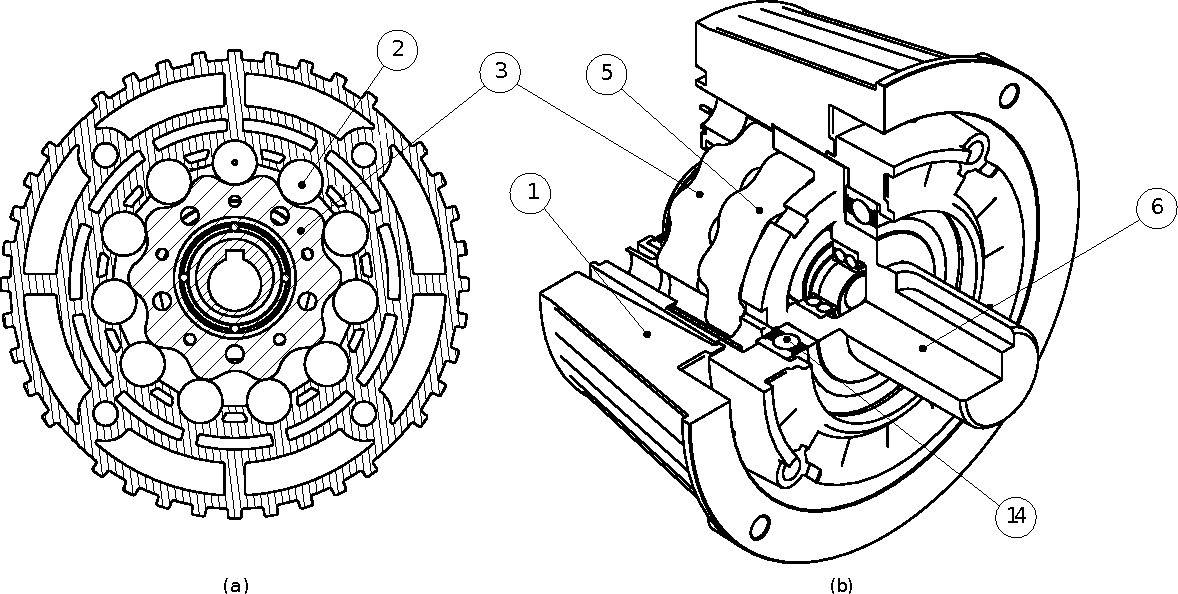
\includegraphics[width=10cm]{\assetsdir/assembly.svg.pdf}
    \end{center}
    \caption[Assemblage mécanique]{\label{assembly}Réducteur cycloïdale de puissance comportant 6. l'axe de sortie, 14. le roulement de sortie, 1. le corps du réducteur en aluminium, 3 et 5. les disques cycloïdaux et 2. les goupilles de prise... D'autres informations liées à la figure elle-même peuvent aussi figurer dans la légende}
\end{figure}

Notez ici que la légende est particulièrement longue. Celle que vous retrouverez dans la table figures est plus courte. La commande \mintinline{latex}{\caption[courte]{longue}} permet de saisir une légende courte pour la table des figures et une légende longue pour documenter la figure. Utilisez \mintinline{latex}{\fig[short=Légende courte]{Légende longue}{fichier}}.

La figure \ref{assembly} est un dessin technique épuré qui permet de décrire un phénomène ou un fonctionnement important dans le rapport technique. Les mises en plan détaillées seront quant à elles disponibles en annexes.

\section{Tableaux}

Concernant les tableaux un seul conseil : restez simple et minimaliste, n'ajoutez des séparateurs que là ou c'est nécessaire pour améliorer la lisibilité. Une liste de quelques cantons suisses est donnée à titre d'exemple dans la table \ref{cantons}.

\begin{table}[h]
    \begin{center}
        \caption{Liste des cantons \label{cantons}}
        \begin{tabular}{c|l|r}
            Abréviation & Nom du canton & Depuis                  \\ \hline
            ZH          & Zürich        & \ordinalnum{1} mai 1351 \\
            BE          & Berne         & 6 mars 1353             \\
            FR          & Fribourg      & 22 décembre 1481        \\
            VD          & Vaud          & 19 février 1815         \\
            VS          & Valais        & 4 août 1815             \\
            NE          & Neuchâtel     & 19 mai 1815             \\
            GE          & Genève        & 19 mai 1815
        \end{tabular}
    \end{center}
\end{table}

Comparez la lisibilté de cette même table avec celle que vous pourriez trouver dans un document Word :

\begin{table}[h]
    \begin{center}
        \caption{Liste des cantons (vilain)}
        \begin{tabular}{|l|l|l|} \hline
            \textbf{Abréviation} & \textbf{Nom du canton} & \textbf{Depuis}         \\
            \Xhline{4\arrayrulewidth}
            ZH                   & Zürich                 & \ordinalnum{1} mai 1351 \\ \hline
            BE                   & Berne                  & 6 mars 1353             \\ \hline
            FR                   & Fribourg               & 22 décembre 1481        \\ \hline
            VD                   & Vaud                   & 19 février 1815         \\ \hline
            VS                   & Valais                 & 4 août 1815             \\ \hline
            NE                   & Neuchâtel              & 19 mai 1815             \\ \hline
            GE                   & Genève                 & 19 mai 1815             \\ \hline
        \end{tabular}
    \end{center}
\end{table}

Si vous devez donner une spécification technique, n'oubliez pas de mentionner les valeurs minimales, maximales et nominales sans omettre l'unité de mesure. Notez que les séparateurs verticaux sont souvent critiqués pour réduire la lisibilité mais parfois ils sont utiles. Utilisez-les avec parcimonie. Jouez avec l'alignment des colonnes pour accroître la lisibilité et utilisez l'environmement \mintinline{latex}{tabularx} pour plus d'unité dans les largeurs de vos tableaux.

\begin{table}[h]
    \begin{center}
        \caption{Exigences techniques \label{specification}}
        \begin{tabularx}{\textwidth}{cXcccr}
            \toprule
            No. & Exigence                                                                   & Min. & Nom. & Max. & Unité                           \\
            \midrule
            E1  & Tension d'alimentation                                                     & 12   & 24   & 48   & \si{\volt}                      \\
            E2  & Fréquence                                                                  & 50   &      & 60   & \si{\hertz}                     \\
            E3  & Concentration                                                              &      & 300  & 1200 & \si{\nano\gram\per\milli\litre} \\
            E4  & \multicolumn{5}{l}{Doit pouvoir être stoppé à l'aide d'un arrêt d'urgence}                                                        \\
            \bottomrule
        \end{tabularx}
    \end{center}
\end{table}

L'exemple de la table \ref{specification}, assigne pour chaque exigence un numéro unique. Cette table est \textbf{normative}, chaque élément doit pouvoir être référencé par un identifiant unique (cf. T\ref{specification}-E3). Dans le cas ou cet identifiant est utilisé en dehors de ce document, la version du document devra être renseignée.

\section{Index}
\LaTeX~ permet d'indexer les mots \index{mots} importants. Il suffit de placer les termes importants d'un paragraphe dans la commande \mintinline{latex}{\index{terme}} et ils apparaîtront automatiquement à la fin de ce rapport dans l'index du document.

\index{Napoléon}

Imaginons que dans cette section nous parlions du cheval blanc \index{cheval blanc} de Napoléon. Il se pourrait que le lecteur recherche ce passage dans la version imprimée du rapport. Avec l'index, rien de plus facile. Allez jeter un oeil à la page \pageref{index}.

\section{Notes de bas de page}

\maraja{Je suis une marginale, et je suis utile pour résumé un paragraphe en quelques mots.} Parfois, il est plus élégant d'annoter une définition en utilisant une note de bas de page \footnote{La note en bas de page (ou note de bas de page) est une forme littéraire, consistant en une ou plusieurs lignes ne figurant pas dans le texte.}. Alternativement il est possible d'annoter un paragraphe avec une note marginale.

\section{Glossaire et acronymes}

La \Gls{heig-vd} membre de la \Gls{hes-so} propose ce modèle de document. Le format \LaTeX~est particulièrement adapté pour les documents qui contiennent des expressions mathématiques. Pour plus de détail sur l'utilisation d'un glossaire, se référer à \href{https://www.overleaf.com/learn/latex/Glossaries}{Overleaf/Glossaires}. Tient donc, ci-dessus nous utilisons deux acronymes. Les trouverez-vous dans le glossaire en page \pageref{glossaire} ?

\section{Unités de mesure}

Lorsque vous mentionnez des quantités, utilisez les unités du système international. \LaTeX~et le paquet \texttt{siunitx} permet la saisie de quantités. La commande suivante permet d'afficher \SI{42.12}{\kilo\gram\metre\per\square\second}.\par

\mintinline{latex}{\SI{42.12}{\kilo\gram\metre\per\square\second}}\par

Notez qu'une espace fine précède l'unité et que ces dernières ne sont pas en italiques.
%%fi

\chapter{Présentation du framework Baremaps}
Le framework Baremaps est constitué de plusieurs modules, certains utilisés par tous les projets utilisant le framework, d'autres n'étant utilisés que par certains projets. Parmi les modules principaux, nous avons les modules \texttt{baremaps-cli}, \texttt{baremaps-core}, \texttt{baremaps-server} ainsi que \texttt{basemap}. Parmi les différents points abordés par ce rapport intermédiaire, seuls ces modules seront concernés. Je ne vais donc pas m'attarder ici sur les autres modules du framework.

\section{baremaps-cli}

Le module \texttt{baremaps-cli} est un module permettant de lancer des commandes en ligne de commande pour effectuer des opérations générales avec le framework Baremaps. Ce module est utilisé pour lancer des commandes telles que l'import de données OpenStreetMap ou le lancement d'un serveur web pour afficher des données OpenStreetMap.

\section{baremaps-core}

Le module \texttt{baremaps-core} est un module regroupant la logique métier du framework Baremaps. Ce module est utilisé pour effectuer des opérations telles que la génération de tuiles vectorielles à partir de données OpenStreetMap. C'est dans ce module que la majorité du code qui me servira et que j'écrirai se trouve.

\section{baremaps-server}

Le module \texttt{baremaps-server} est le module qui se charge de lancer un serveur web pour afficher des données OpenStreetMap. Ce module comporte donc les ressources nécessaires pour construire la page web affichant les données OpenStreetMap. C'est dans ce module que Cesium JS sera utilisé et configuré.

\section{basemap}
\label{sec:basemap}

Le module \texttt{basemap} est le module permettant de'importer le fichier OpenStreetMap et de le transformer en une base de données PostgreSQL/PostGIS. À l'heure ou j'écris ce rapport, je n'ai pas encore eu à travailler sur ce module.

\section{Fondements écrits par Antoine Drabble}

Afin d'évaluer si le projet s'apprêtais à être utilisé dans le cadre d'un travail de Bachelor, M. Antoine Drabble a effectué un travail de recherche et a produit un prototype de visualisation de bâtiments 3D à l'intérieur du client Cesium JS sur lequel je vais m'appuyer. Ce prototype, bien qu'incomplet, pose les fondements de l'utilisation de Cesium JS, la spécification 3D Tiles et le framework Baremaps les uns avec les autres. Ce prototype est donc un bon point de départ pour mon travail.

Il n'est pas pertinent de détailler ici le travail effectué par M. Antoine Drabble fichier par fichier mais j'expliquerai au fur et à mesure de ce rapport ce qui a été fait et ce que je dois modifier ou ajouter pour remplir mes objectifs.

\chapter{Utilisation de la base de donnée OpenStreetMap}
Comme décrit en page \pageref{sec:basemap} \autoref{sec:basemap}, le module Basemap se charge d'importer le fichier OpenStreetMap et de le transformer en une base de données PostgreSQL/PostGIS. Une fois la base de donnée générée, il faut maintenant pouvoir récupérer et traiter les données correctement.

\newpage

\section{Extraction des données et définition d'un bâtiment}
\label{sec:extraction}

La partie nous intéressant dans la base de données OpenStreetMap est la table \texttt{osm\_nodes}. Cette table contient les données de tout les bâtiments. Ceux-ci ne contiennent généralement qu'une \Gls{géométrie}, une structure de donnée contenant plusieurs points et formant un polygone. Parfois seulement, des \Gls{tags} peuvent être ajoutés. Ces tags peuvent contenir des informations sur la hauteur du bâtiment, sa couleur, son matériau, etc.

La \href{https://wiki.openstreetmap.org/wiki/Simple_3D_Buildings}{documentation OpenStreetMap}\footnote{https://wiki.openstreetmap.org/wiki/Simple\_3D\_Buildings} nous permet d'avoir la liste complète des tags existants et nous intéressant concernant les bâtiments.

Pour pouvoir récupérer toutes ces informations, j'utilise la requête SQL suivante :

\begin{verbatim}
SELECT st_asbinary(geom),
    tags -> building,
    tags -> height,
    tags -> building:levels,
    tags -> building:min_level,
    tags -> building:colour,
    tags -> building:material,
    tags -> building:part,
    tags -> roof:shape,
    tags -> roof:levels,
    tags -> roof:height,
    tags -> roof:color,
    tags -> roof:material,
    tags -> roof:angle,
    tags -> roof:direction,
    tags -> amenity
FROM osm_ways
WHERE (tags ? building or tags ? building:part) and
    st_intersects(geom, st_makeenvelope(%1$s, %2$s, %3$s, %4$s, 4326))
LIMIT %5$s;
\end{verbatim}

\texttt{\%1\$s, \%2\$s, \%3\$s, \%4\$s, et \%5\$s} sont des espaces réservés qui seront remplacés par les coordonnées de la zone à charger lors de l'exécution de la requête.

\newpage

\section{Couleurs des bâtiments}

Concernant la couleur des bâtiments, il est possible de récupérer la couleur de base du bâtiment en utilisant le tag \texttt{building:colour}. Cependant, ce tag ne donne que le mot en anglais de la couleur et non pas son code RGB, HEX ou HSL.

Pour remédier à cela, j'ai créé la classe \texttt{ColorUtils}\footnote{baremaps-core/src/main/java/org/apache/baremaps/tdtiles/utils/ColorUtility.java} qui contient une map statique de toutes les couleurs selon le standard définit par \href{https://www.w3schools.com/cssref/css_colors.php}{W3Schools}\footnote{https://www.w3schools.com/cssref/css\_colors.php}. Cette classe permet de convertir le nom de la couleur en code HEX :

\begin{lstlisting}[style=java]
public class ColorUtility {
  private static final Map<String, String> colorMap;

  static {
    colorMap = new HashMap<>();
    colorMap.put("aliceblue", "f0f8ff");
    // ...
    colorMap.put("yellowgreen", "9acd32");
  }

  public static Color parseName(String color) {
    // Calcul des valeurs RGB en fonction du code HEX.
    return new Color(r, g, b);
  }
}
\end{lstlisting}

\texttt{Color}\footnote{baremaps-core/src/main/java/org/apache/baremaps/tdtiles/utils/Color.java} étant un record, il est possible de créer une nouvelle couleur en passant les valeurs RGB en paramètre.

Une fois la couleur RGB récupérée, il est possible de l'utiliser dans la classe \texttt{GltfBuilder}\footnote{baremaps-core/src/main/java/org/apache/baremaps/tdtiles/GltfBuilder.java} pour donner la couleur au bâtiment lors de sa modélisation.

\newpage

\section{Hauteur des bâtiments}

Le calcul de la hauteur des bâtiments doit se faire en fonction de la \href{https://wiki.openstreetmap.org/wiki/Simple_3D_Buildings}{définition}\footnote{https://wiki.openstreetmap.org/wiki/Simple\_3D\_Buildings} des bâtiments par OSM. Si aucun tags ne donne la hauteur du bâtiment, il aura par défaut une hauteur de 10 mètres.

Sinon, la hauteur du bâtiment est calculée en fonction des tags \texttt{height}, \texttt{building:levels}, \texttt{building:min\_level}, \texttt{roof:height} et \texttt{roof:levels} :

\begin{itemize}
    \item On commence avec une hauteur de bâtiment de 0 mètres.
    \item Si aucun tag n'est présent,
          \begin{itemize}
              \item La hauteur du bâtiment est de 10 mètres.
          \end{itemize}
    \item Sinon, si le tag \texttt{height} est présent,
          \begin{itemize}
              \item La hauteur du bâtiment est égale à la valeur du tag \texttt{height}.
              \item Si le tag \texttt{roof:height} est présent,
                    \begin{itemize}
                        \item La hauteur du toit \texttt{roof:height} doit être soustraite de la hauteur du bâtiment
                    \end{itemize}
          \end{itemize}
    \item Sinon,
          \begin{itemize}
              \item Si le tag \texttt{building:levels} est présent,
                    \begin{itemize}
                        \item La hauteur du bâtiment est égale à la valeur du tag \texttt{building:levels} multipliée par 3 mètres.
                    \end{itemize}
              \item Si le tag \texttt{roof:levels} est présent,
                    \begin{itemize}
                        \item La hauteur du toit \texttt{roof:levels} multipliée par 3 mètres doit être additionnée à la hauteur du bâtiment.
                    \end{itemize}
              \item Si le tag \texttt{building:min\_level} est présent,
                    \begin{itemize}
                        \item La hauteur du vide en dessous du bâtiment est égale à la valeur du tag \texttt{building:min\_level} multipliée par 3 mètres.
                    \end{itemize}
          \end{itemize}
\end{itemize}

La hauteur connue, on peut la transmettre à la classe \texttt{GltfBuilder}\footnote{baremaps-core/src/main/java/org/apache/baremaps/tdtiles/GltfBuilder.java} pour donner la hauteur au bâtiment lors de sa modélisation.

\newpage

\section{Géométries des bâtiments}

La classe \texttt{GltfBuilder} a donc accès à la couleur et à la hauteur du bâtiment. Ces informations ainsi que les autres tags lui sont transmis à travers le record \texttt{Building}\footnote{baremaps-core/src/main/java/org/apache/baremaps/tdtiles/building/Building.java} et \texttt{Roof}\footnote{baremaps-core/src/main/java/org/apache/baremaps/tdtiles/building/Roof.java}.

Outre ces informations, \texttt{Building} comporte aussi une \texttt{Geometry}\footnote{org.locationtech.jts.geom.Geometry} qui nous sert à déterminer le polygone au sol du bâtiment. Grâce à ce polygone, nous pouvons extruder le bâtiment en 3D. Cependant une \texttt{Geometry} ne contient qu'une liste de points et il faut une liste de triangles pour pouvoir modéliser le bâtiment en 3D. Pour cela, la méthode \texttt{DelaunayTriangulationBuilder}\footnote{org.locationtech.jts.triangulate.DelaunayTriangulationBuilder} était utilisée. Le problème était que la \href{https://en.wikipedia.org/wiki/Delaunay_triangulation}{\textit{Delaunay triangulation}}\footnote{https://en.wikipedia.org/wiki/Delaunay\_triangulation} ne fonctionne pas avec des polygones concaves. Une version complémentaire de cette méthode est la \href{https://en.wikipedia.org/wiki/Constrained_Delaunay_triangulation}{\textit{Constrained Delaunay triangulation}}\footnote{https://en.wikipedia.org/wiki/Constrained\_Delaunay\_triangulation} qui fonctionne avec des polygones concaves en définissant des segments comme bords du polygone. Cette version de l'algorithme est aussi disponible dans la librairie \href{https://locationtech.github.io/jts/}{JTS}\footnote{https://locationtech.github.io/jts/} mais elle propose aussi la classe \href{https://locationtech.github.io/jts/javadoc/org/locationtech/jts/triangulate/polygon/PolygonTriangulator.html}{\texttt{PolygonTriangulator}}\footnote{https://locationtech.github.io/jts/javadoc/org/locationtech/jts/triangulate/polygon/PolygonTriangulator.html} qui permet aussi de faire une triangulation de polygones concaves de manière moins optimisée mais plus rapide que la \textit{Constrained Delaunay triangulation}. C'est donc cette classe que j'ai utilisée pour trianguler les bâtiments.

Grâce à cette nouvelle triangulation, il est possible de modéliser les bâtiments en 3D correctement, même ceux comprenant des cours intérieures ou des trous dans leur structure.

La classe \texttt{DelaunayTriangulationBuilder} comportait cependant un paramètre \texttt{tolerance} qui permettait de définir la distance minimale entre deux points afin d'optimiser le coût de la triangulation. Cette possibilité n'est pas disponible dans la classe \texttt{PolygonTriangulator}, néanmoins j'implémente une alternative dans le chapitre suivant.

\chapter{Optimisation de l'affichage des bâtiments}
\label{chap:optimisation}
Le plus gros problème lors de l'utilisation de l'application actuellement est que lorsque l'on déplace la caméra dans une nouvelle zone de la carte, les bâtiments prennent parfois plus d'une dizaine de secondes à s'afficher tout en bloquant le site web. De plus, les bâtiments apparaissent de manière à priori aléatoire et non au plus proche de la caméra.

Je vais, dans ce chapitre, aborder différentes possibilités d'optimisation.

\newpage
\section{Implicit tiling}
\label{sec:implicit-tiling}

Avant de chercher à optimiser l'affichage des bâtiments, il est important de comprendre comment les bâtiments sont actuellement affichés. La procédure entière comporte plusieurs étapes. Le client Cesium JS commence par charger le fichier \texttt{tileset.json}\footnote{baremaps-server/src/main/resources/tdtiles/tileset.json} qui contient les informations sur la manière dont il doit charger les tuiles. Parmi ces informations, on trouve les URI auxquelles il doit envoyer des requêtes pour obtenir les tuiles mais aussi les informations nécessaires à définir l'\texttt{implicit tiling} :

\begin{verbatim}
"implicitTiling" : {
    "subdivisionScheme" : "QUADTREE",
    "subtreeLevels" : 6,
    "availableLevels" : 18,
    "subtrees" : {
        "uri" : "/subtrees/{level}.{x}.{y}.json"
    }
}
\end{verbatim}

L'\Gls{implicit tiling} est une technique qui consiste à diviser la carte en tuiles de manière récursive. Tant que le \texttt{level} de division n'a pas atteint la valeur maximum \texttt{availableLevels}, on divise la tuile dans laquelle nous nous trouvons en quatre tuiles de même taille. On peut voir un exemple de cette division sur la figure \ref{quadtree.pdf}.

\fig[H, width=1\textwidth]{Exemple de quadtree utilisé par Cesium JS}{quadtree.pdf}

\newpage
La notion de \texttt{levels} est directement liée au \texttt{quadtree} lui même. À chaque division, le \texttt{level} augmente de 1. Ainsi, une tuile de \texttt{level} 0 est la tuile de base, une tuile de \texttt{level} 1 est une tuile résultant de la division de la tuile de \texttt{level} 0, etc. Nous trouverons donc les tuiles de \texttt{level} le plus élevé à l'endroit où nous nous trouvons.

Sachant cela, nous pouvons maintenant comprendre comment les bâtiments sont affichés. Lorsque le client Cesium JS charge une tuile, il envoie une requête au serveur Baremaps pour obtenir les bâtiments de cette tuile. Le serveur Baremaps va alors vérifier que le \texttt{level} de la tuile est suffisamment élevé pour que les bâtiments soient affichés. Si tel est le cas, il va alors effectuer la requête SQL vu au chapitre \ref{sec:extraction} avec néanmoins une limite au nombre de bâtiments retournés (ce nombre dépendant du \texttt{level}). Les bâtiments retournés sont alors convertit en \texttt{glTF} et envoyés au client Cesium JS qui les affiche.

Cette approche est la source du problème causant les bâtiments à s'afficher de manière ressemblant à de l'aléatoire. Si nous imposons une limite de bâtiments par tuile, alors la requête SQL ne retournera que les premiers bâtiments dans sa liste, peu importe qu'ils soient proches de la caméra ou non.

J'ai donc modifié ce fonctionnement pour que lorsqu'une tuile soit demandée à être affichée, le serveur Baremaps retourne tous les bâtiments de cette tuile. Néanmoins, un changement est donc aussi nécessaire quand à quelle tuile doit être affichée ou non. Générer tous les bâtiments d'une tuile trop grande ne fera que bloquer le client Cesium JS le temps quel la tuile lui soit fournie. En augmentant le \texttt{level} à partir duquel les bâtiments sont affichés, nous pouvons garantir que tous les bâtiments affichés sont proches de la caméra tout en évitant de prendre trop de temps à les générer.

\newpage
\section{Profiling}

Afin de voir exactement quelle partie du code bloque lorsque l'on déplace la caméra, j'ai utilisé l'outil de \texttt{profiling} lié à l'IDE IntelliJ. Cet outil permet de voir le temps passé dans chaque méthode du code. J'ai donc lancé le \texttt{profiler} et j'ai déplacé la caméra dans une zone de la carte où les bâtiments mettent du temps à s'afficher. Les résultats sont visibles sur la figure \ref{profiling.pdf}.

\fig[H, width=1\textwidth]{Résultats du profiling}{profiling.pdf}

Grâce à ces résultats, nous pouvons observer que c'est l'écriture en fichiers binaire \texttt{glTF} des bâtiments qui prend le plus de temps. Malheureusement, cette fonction \texttt{writeBinary}\footnote{de.javagl.jgltf.model.io.v2.GltfAssetWriterV2} ne peut pas être plus optimisée que ce qu'elle est déjà. Je parle néanmoins dans la section suivante d'une manière de lui alléger la tâche.

On remarque aussi que la méthode \texttt{createNode}\footnote{baremaps-core/src/main/java/org/apache/baremaps/tdtiles/GltfBuilder.java} prend aussi beaucoup de temps. Ici il est possible de \textit{multithreader} cette méthode pour gagner du temps. J'ai donc écrit la méthode \texttt{createNodes}\footnote{baremaps-server/src/main/java/org/apache/baremaps/server/TdTilesResources.java} qui permet de le faire en prenant en compte le nombre de CPUs disponibles.

\newpage
\section{Système de compression des géométries des bâtiments}

Comme vu à la section précédente, l'écriture des bâtiments en fichiers binaires \texttt{glTF} est une des étapes les plus longues. Une manière de réduire le temps passé dans cette étape est de simplement réduire la quantité de donnée que la fonction prend en paramètre. Pour cela, j'utilise un système de \textit{Level of details} (LOD) pour les géométries des bâtiments.

Ce système se base sur les \texttt{levels} des tuiles discutés au chapitre \ref{sec:implicit-tiling}. Plus le \texttt{level} est élevé, plus les bâtiments sont proches de la caméra et donc plus les bâtiments doivent être détaillés. En fonction du \texttt{level} de leur tuile, les bâtiments subissent jusqu'à 3 niveau de compression :

\begin{itemize}
    \item \texttt{level} 0 : Les bâtiments sont affichés en 3D avec toutes les géométries.
    \item \texttt{level} 1 : Les bâtiments sont affichés en 3D avec une géométrie simplifiée.
    \item \texttt{level} 2 : Les bâtiments sont affichés en 2D.
    \item \texttt{level} 3 : Les bâtiments sont affichés en 3D avec toutes les géométries uniquement si ils ont des caractéristiques spécifiques enregistrées dans la base de données OpenStreetMap.
\end{itemize}

Pour visualiser les différences entre les niveaux de compression, je vous invite à regarder la figure \ref{levelsofdetails.pdf} où chaque niveau de détail est simbolisé par une couleur :

\begin{itemize}
    \item \texttt{level} 0 : rouge
    \item \texttt{level} 1 : vert
    \item \texttt{level} 2 : bleu
    \item \texttt{level} 3 : blanc
\end{itemize}

\fig[H, width=1\textwidth]{Niveaux de détails des bâtiments}{levelsofdetails.pdf}

Faire ainsi permet de réduire drastiquement le temps passé à générer ces bâtiments tout en gardant une qualité d'affichage correcte.


\chapter{Conclusion}
%%if
Bien que non nécessaire dans un rapport de Bachelor, la discussion finale d'un projet résume les résultats obtenus et dresse une conclusion objective du projet. Un manager de société est souvent amené à lire de nombreux rapport, il ne s'intéresse généralement qu'à l'introduction au contexte de l'étude et à sa conclusion.

Si nécessaire, n'hésitez pas à scinder votre conclusion en deux parties : une conclusion technique et une conclusion personnelle.

Il est de coutume de signer la conclusion...
%%fi

\vfil
\hspace{8cm}\makeatletter\@author\makeatother\par
\hspace{8cm}\begin{minipage}{5cm}
    %%if
    % Place pour signature numérique
    \printsignature
    %%fi
\end{minipage}

\clearpage
\printbibliography

\appendix
\appendixpage
\addappheadtotoc

%%if
% \chapter{Première annexe}

% Les annexes n'ont pas un contenu \underline{normatif} mais \underline{descriptif}. Tout contenu annexé ne doit pas être nécessaire à la bonne compréhension du travail.

% Les annexes contiennent généralement :

% \begin{itemize}
%     \item les dessins mécaniques (mises en plan);
%     \item les schémas électriques détaillés;
%     \item des photographies du projet;
%     \item des scripts et des extraits de code source;
%     \item des documents techniques \pex \emph{datasheet};
%     \item des développements mathématiques.
% \end{itemize}
% \section{Sous section}
% \lipsum[1]
%%fi

\let\cleardoublepage\clearpage
\backmatter

\label{glossaire}
\printnoidxglossary
\label{index}
\printindex

% Le colophon est le dernier élément d'un document qui contient des notes de l'auteur concernant la mise en page et l'édition du document : il est parfaitement optionnel.
%%if
\clearpage
\Large\textbf{Colophon :}\par\normalsize
\thispagestyle{empty}
La qualité de cet ouvrage repose que le moteur \LaTeX. La mise en page et le format sont inspirés d'ouvrages scientifiques tels que le modèle de thèse de l'EPFL et celui des publications O'Reilly.

Les diagrammes et les illustrations sont édités depuis l'outil en ligne draw.io. Certaines illustrations ont été reprises dans Adobe Illustrator. Les représentations 3D sont exportées de SolidWorks et certains graphiques sont générés à la volée depuis un code source Python.

L'auteur fictive de ce document \emph{Maria Bernasconi} est un nom emprunté, par amusement, aux spécimens publiés par Postfinance.

Ce document a été compilé avec XeLaTeX.

La famille de police de caractères utilisée est \emph{Computed Modern} créée par Donald Knuth avec son logiciel METAFONT.
\vfil
Le Colophon est le dernier élément d'un document qui contient des notes de l'auteur concernant la mise en page et l'édition du document : il est parfaitement optionnel.
%%fi

\end{document}